\chapter{Detailed Airside Component Design}
\label{ch:Detailed Airside Component Design}

\section{Structure of the Airside Subsystem}
\label{sec:Structure of the Airside Subsystem}

A critical first step in the airside subsystem design process was the creation of a testing environment that could contain all of the components discussed in Section \ref{sec:Explanation of Facility Operation}. Since the airside subsystem is large and will experience testing under a wide range of operating conditions, it is appropriate to list the most critical items to be addressed in the design process. These include being airtight, being resistant to rusting, minimizing external condensation during low temperature testing, and being able to support its own weight safely.

A local HVAC unitary equipment manufacturer, AAON, Inc., designs and builds rooftop air conditioning units using galvanized sheet metal panels filled with polyurethane spray foam insulant. Cremaschi and Lee (2008) completed a heat transfer analysis on these panels when constructing a similar facility. Their study found that 4 in thick panels provide adequate insulation to the surrounding room air temperature and prevent external surface condensation down to -20\degree F. Additionally, the study results suggest the insulating value of 4 in thick panels is sufficient for continuous operation. The space between panels is occupied by a neoprene foam tape to create the required airtight seal. With this information in mind, the galvanized steel panels manufactured by AAON are an ideal candidate for construction of the airside subsystem.

The base of the airside subsystem was the first part of the structure designed. The base is of critical importance since it acts as the foundation for the remainder of the structure. It should be noted that the construction of the facility took place in a room (ATRC 041/043) with a slanted floor. This was originally done to allow for drainage. Due to this, a method to level the base of the airside subsystem was developed. Since leveling the floor of ATRC 041/043 was not a viable option due to facilities management limitations, elevating the base of the airside subsystem with a rail type system along with leveling steel plate shims became the preferred leveling method. Figure \ref{fig:RailDescription} shows an example rail. The rails are composed of two bent sheet metal pieces and are manufactured in 7 ft increments. Rail segments are connected together using a "seam splice" and self drilling screws. Two parallel rails can be used to support the ends of a base panel and elevate the airside subsystem off the floor by approximately 4 in.

\begin{figure}[h]
\centering
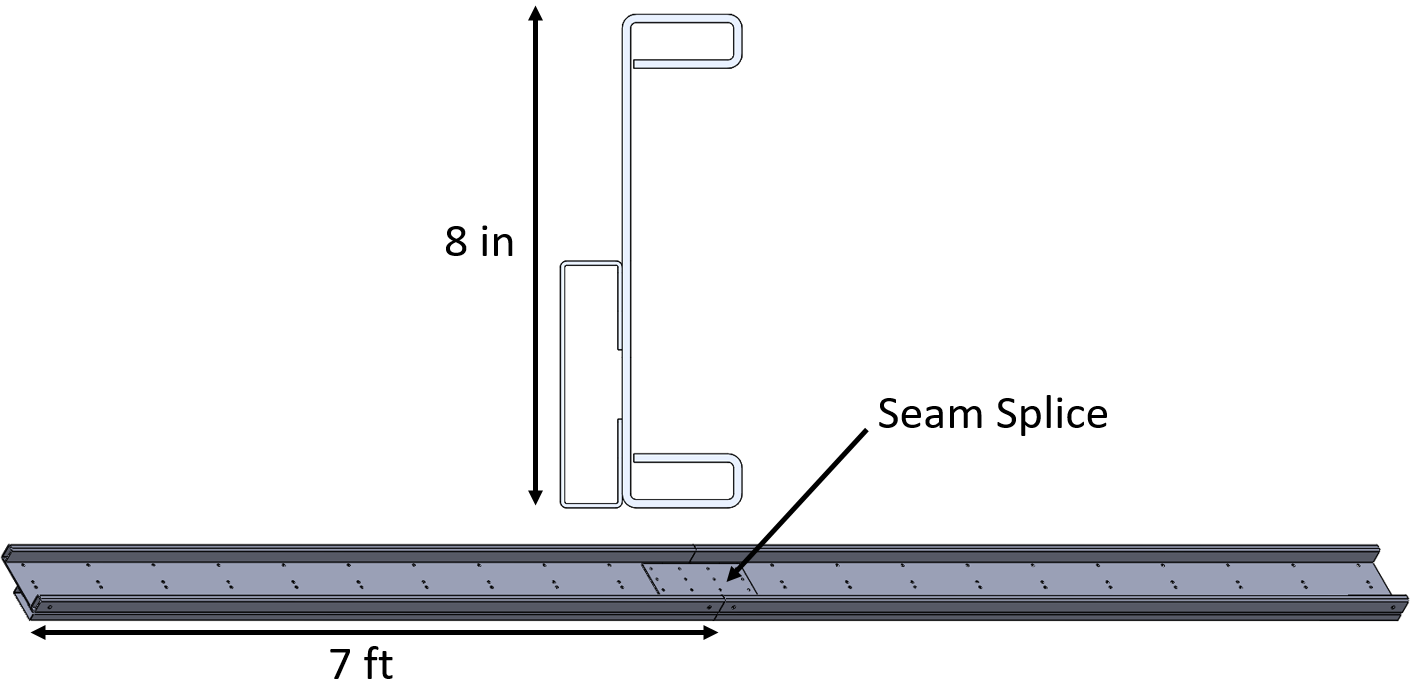
\includegraphics[width=1\textwidth]{RailCrossSectionAndIsoView}
\caption{Top: Cross sectional view of base rail. Bottom: Isometric view of conjoining rails (cross sectional view on the left end).}
\label{fig:RailDescription}
\end{figure}

While the rails allow an elevated base to be assembled easily, manufacturing limitations did not allow for full width (12 ft) base panels. Because of this, the base was split into two sections, the test section and conditioning section, to shorten the overall length of individual panels. Test section panels are 88 in long by 18 in wide while conditioning section panels are 52 in long by 24 in wide. Both panels are simple rectangular prisms. This of course introduces a new issue; how to support the point where the test section and conditioning panels meet. To solve this issue, 4 in square by 1/4 in thick structural tubing was used as a support at this meeting point. S channel bends and rivets were used to connect 7 ft long sections of tubing together. Figure \ref{fig:BaseIsoAndCrossView} shows how panels will be placed on the parallel railing. This arrangement is repeated for the 42 ft length of the airside subsystem. Self drilling screws are used to attach panels to the standard rails and rivets are used to attach panels to the S channel bend of the structural tubing. Panels are screwed to each other using strips of sheet metal called "splices". Lastly, the open space between the floor of ATRC 041/043 and the base is blanked off to block entry into the small space underneath the facility. Figure \ref{fig:FinalBase} shows the completed base assembly. 

\begin{figure}[h]
\centering
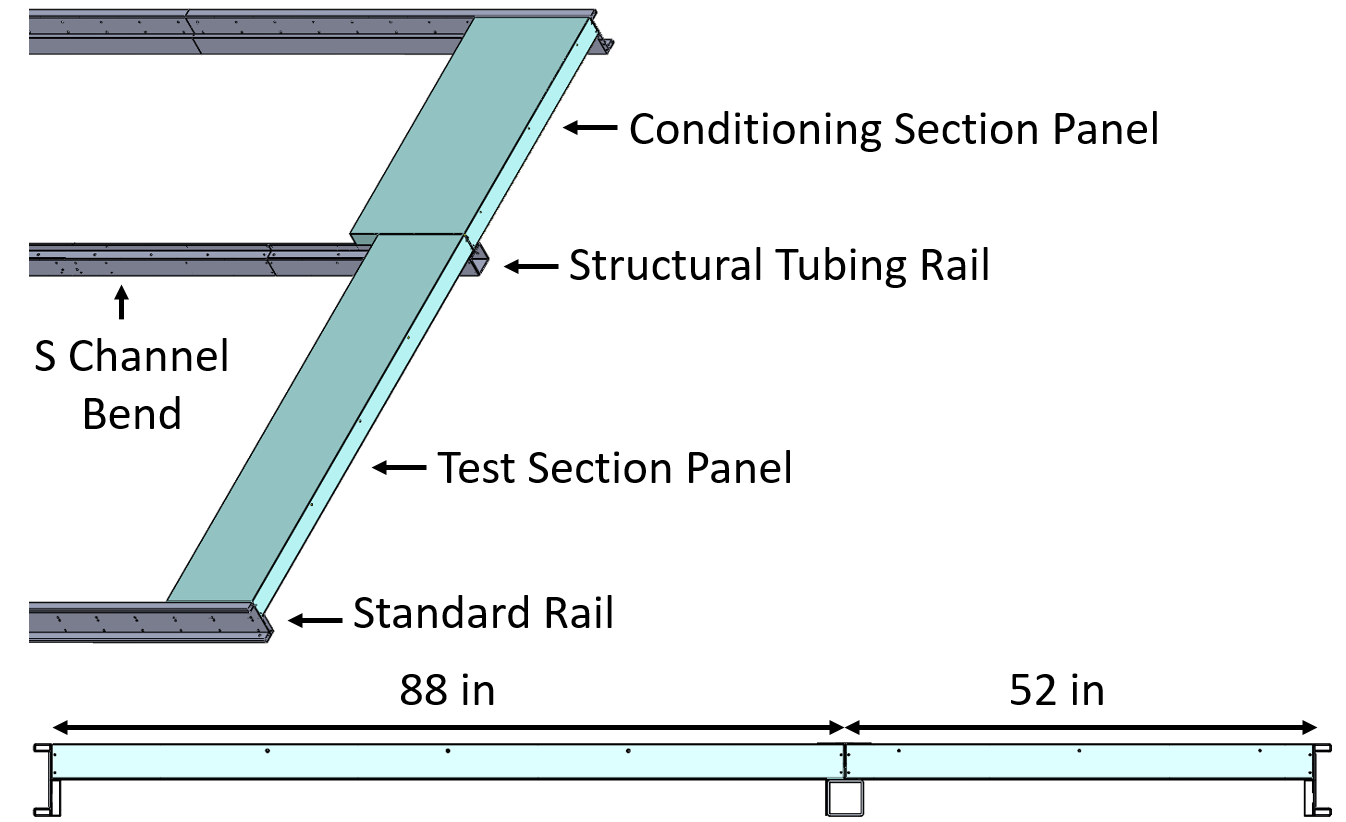
\includegraphics[width=1\textwidth]{BaseIsoAndCrossView}
\caption{Top: View of parallel rails with both types of base panels. Bottom: Cross sectional view of rails with base panels.} 
\label{fig:BaseIsoAndCrossView}
\end{figure}

\begin{figure}[h!]
\centering
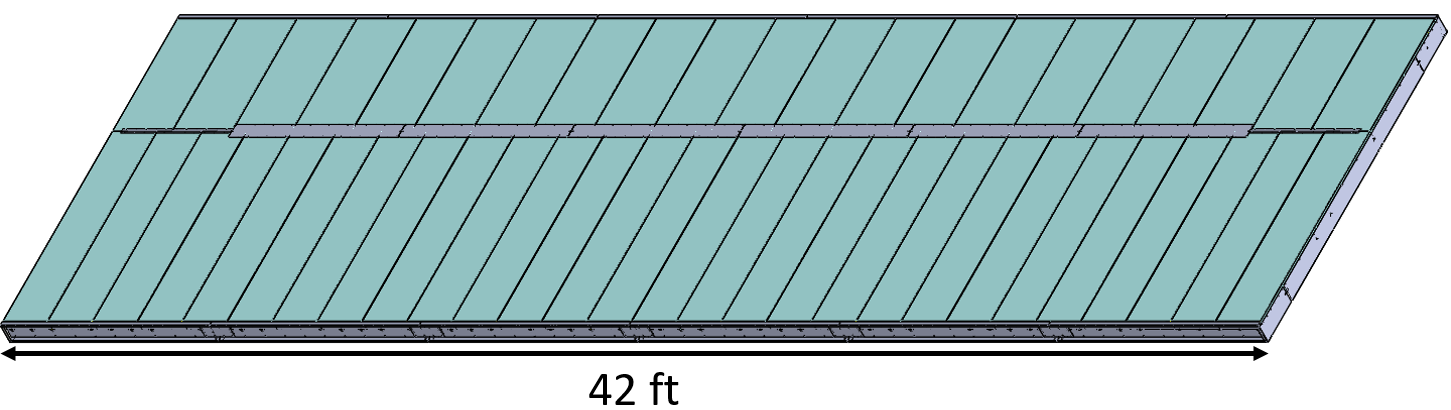
\includegraphics[width=1\textwidth]{FinalBase}
\caption{Completed airside subsystem base} 
\label{fig:FinalBase}
\end{figure}

\FloatBarrier

With the base designed, the design of walls, doors, and access panels was the next logical step. Wall panels are similar to base panels, but have some key differences. In general there are two types of wall panels: external and internal. External wall panels can be further broken down into two distinct groups: flat top and step top panels. 96 in tall flat top panels are used on the short base edge while 98 in tall (maximum height) step top panels are used along the long base edge. All flat top panels are 17 in width while step top panels come in a variety of widths, ranging from 18 in to 48 in. This combination of different top styles helps to support roof panels and will be discussed in more detail shortly. Small sheet metal flanges at the bottom of each external wall panel panel are screwed to the base. Wall panels are then screwed to one another on the external side of the walls using sheet metal splices. Figure \ref{fig:ExternalWallCorner} shows a corner of the external walls and highlights key features of the panels.

Solid wall panels like those seen in Figure \ref{fig:ExternalWallCorner} are the most common seen with the airside subsystem. However, a need for general viewing and maintenance access was identified, along with a desire to test for maldistribution using PIV (particle image velocimetry) in the future. To satisfy this need, walk though doors and removable access panels were designed that require step top wall panels with openings to pass through. An example door and access panel can be seen in Figure \ref{fig:DoorAndAccessPanelExample}. Each door is 67 in tall by 30 in wide and is equipped with a locking mechanism that prevents the door from opening when latched. Access panels come in a variety of sizes and are bolted to their corresponding wall panel using riv-nuts. 

\begin{figure}
\centering
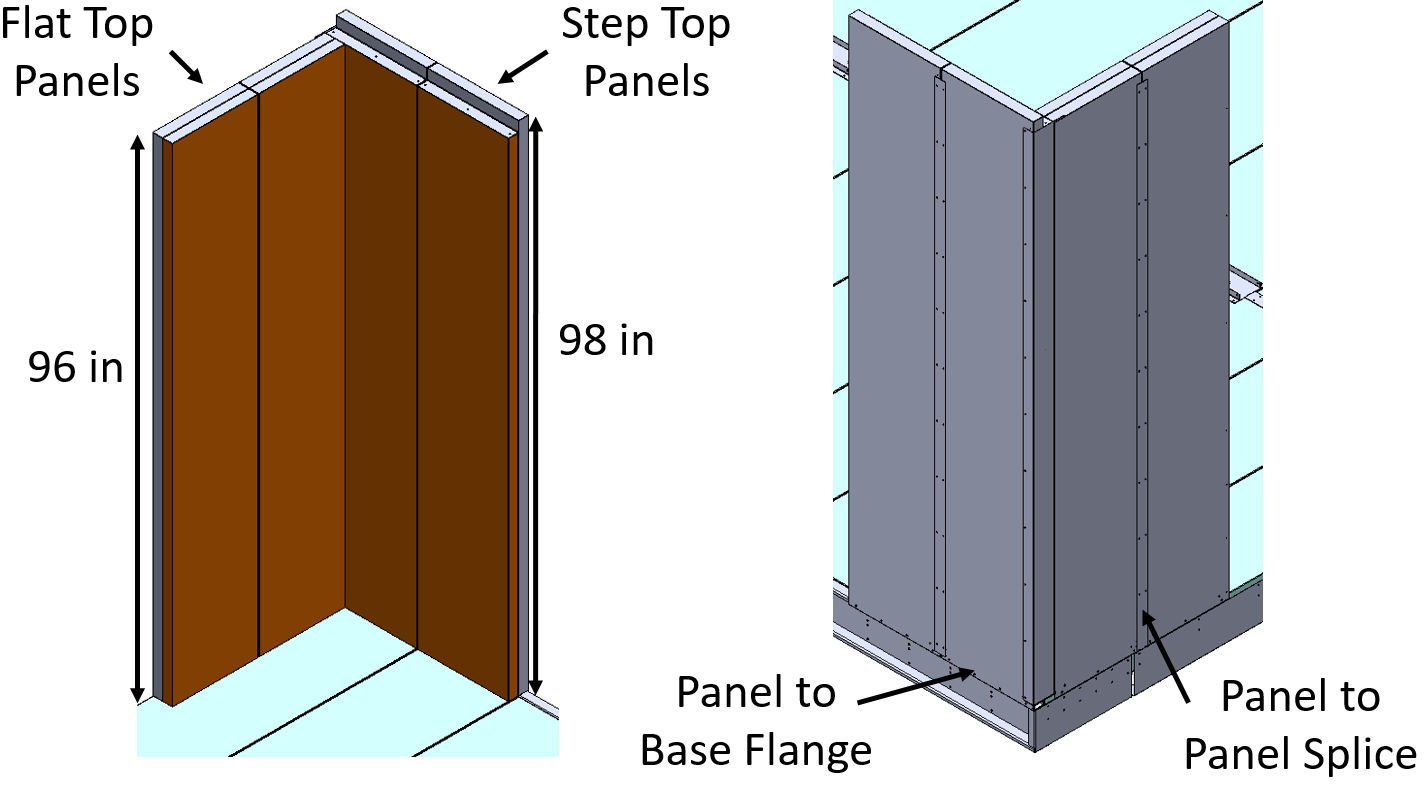
\includegraphics[width=1\textwidth]{ExternalWallCorner}
\caption{Left: Internal view of external wall corner. Right: External view of external wall corner.}
\label{fig:ExternalWallCorner}
\end{figure}

\begin{figure}
\centering
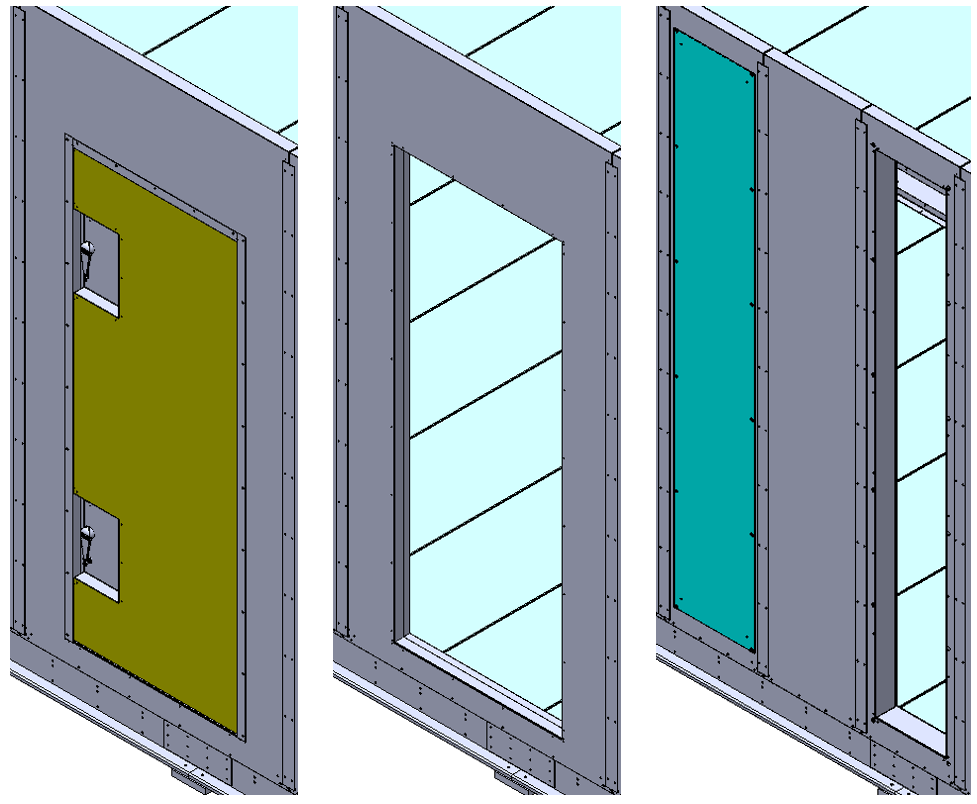
\includegraphics[width=0.75\textwidth]{DoorAndAccessPanelExample}
\caption{From left to right: Wall panel with closed door, wall panel with opening for door, access panel inside wall panel, wall panel with opening for access panel.}
\label{fig:DoorAndAccessPanelExample}
\end{figure}

\FloatBarrier

While external walls are used to insulate the testing environment from the ambient conditions of ATRC 041/043, internal walls are used to partition the test and conditioning sections from one another. Internal wall panels are similar to base panels in that each panel is a simple rectangular prism. The bottom of each internal panel is screwed to the base of the airside subsystem with angle brackets and panels are screwed to each other with splices. Door panels of the same style previously discussed are also implemented into the internal wall panels. Internal wall panels are all 24 in wide, excluding those with doors, and can be 96 in or 98 in tall. The 96 in tall panels were designed to support the roof panels above the area where air travels from the test section to the conditioning section and vice versa. An example of each type of internal wall panel can be seen in Figure \ref{fig:InternalWallExample}. 

\begin{figure} [h!]
\centering
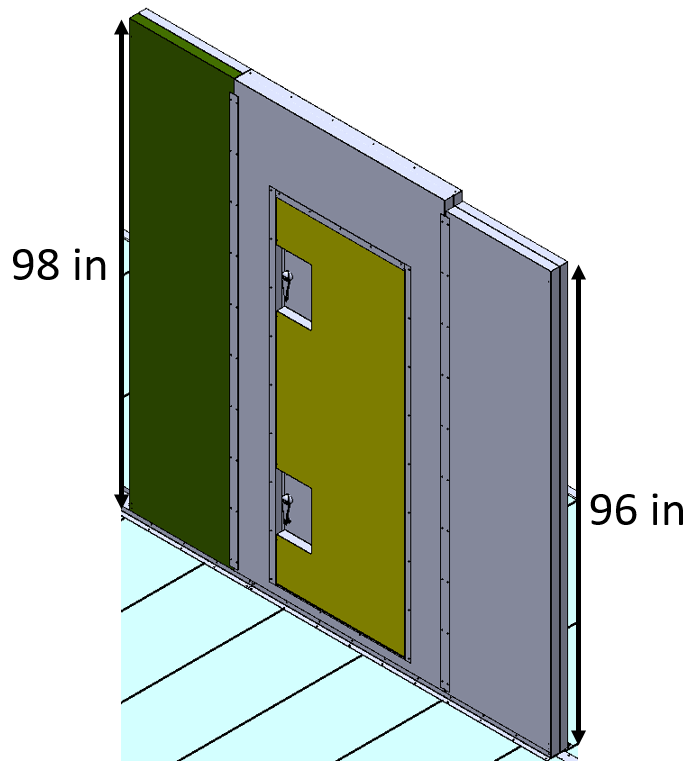
\includegraphics[width=0.5\textwidth]{InternalWallExample}
\caption{From left to right: 98 in tall internal wall panel, internal wall panel with door, and 96 in tall internal wall panel.}
\label{fig:InternalWallExample}
\end{figure}

To conclude, a collection of internal and external wall panels were positioned to allow for access of important airside components, general viewing of the airside subsystem, and PIV testing. The completed arrangement of wall panels can be seen in Figures \ref{fig:CabinNoRoof} and \ref{fig:CabinNoRoof2}. Doors and access panels are highlighted and serve various purposes. Both access panels on the external wall in Figure \ref{fig:CabinNoRoof} will be used for PIV while the access panel on the internal wall is used to service air filters. In Figure \ref{fig:CabinNoRoof2}, from left to right on the external wall, the access panels are for: damper actuator access, electric heater and fan motor access, fan wheel and post conditioning coil damper access, damper actuator access, and conditioning coil access. There is also an opening designated for the steam injection manifold. Red colored doors open outward (into the page) and yellow colored doors open inward (out of the page). 

\begin{figure} [h!]
\centering
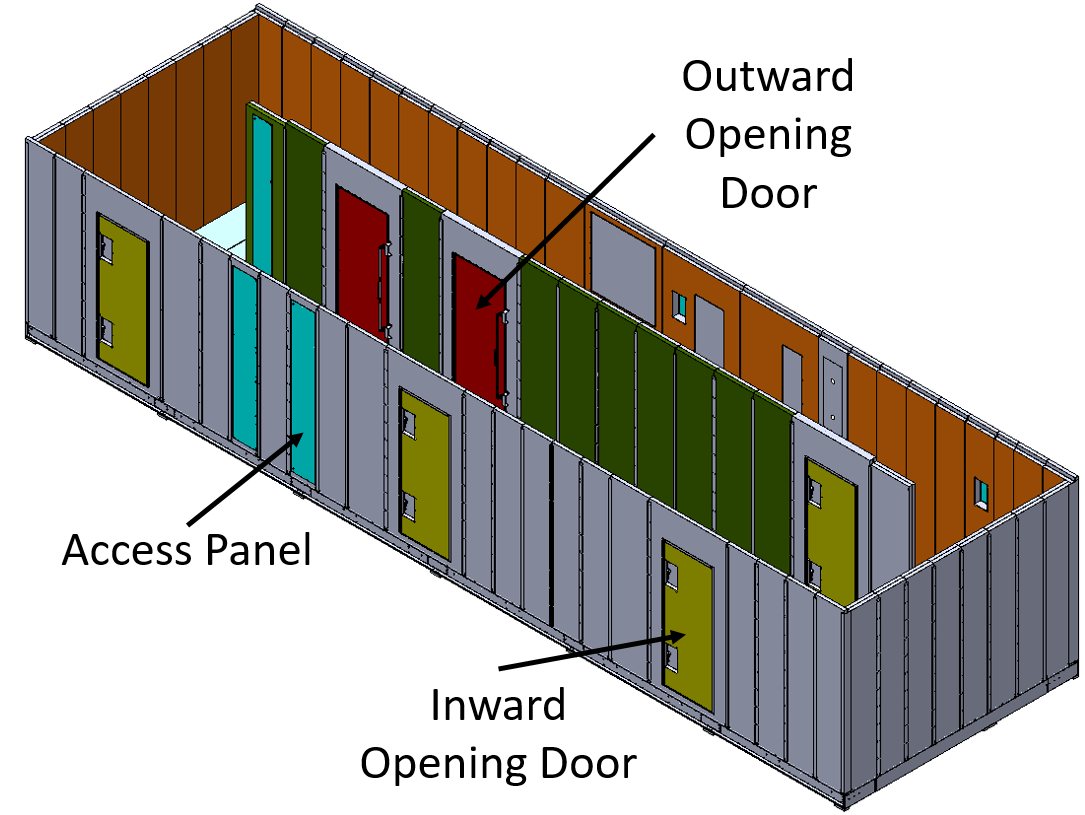
\includegraphics[width=0.85\textwidth]{CabinNoRoof}
\caption{Final arrangement of external and internal airside subsystem walls.}
\label{fig:CabinNoRoof}
\end{figure}

\begin{figure} [h!]
\centering
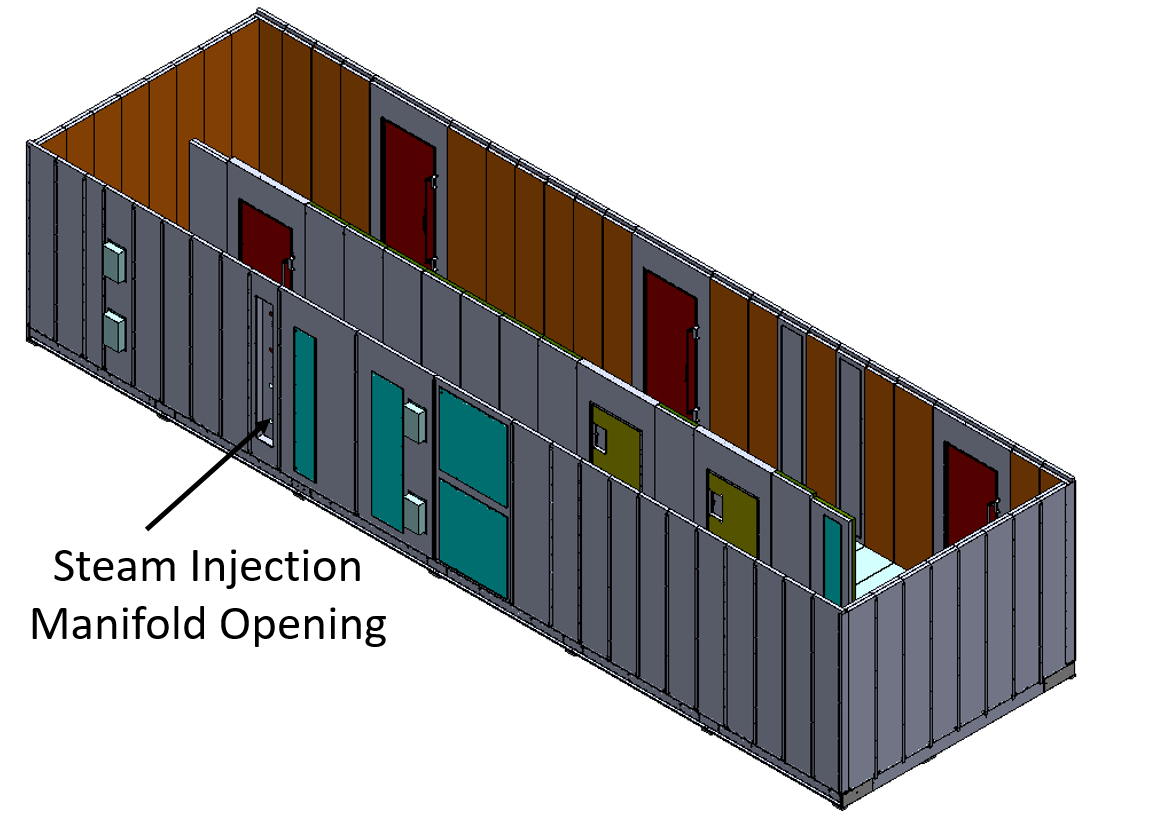
\includegraphics[width=1\textwidth]{CabinNoRoof2}
\caption{Another view of the previous figure.}
\label{fig:CabinNoRoof2}
\end{figure}

\FloatBarrier

The final structural component designed was the roof. Roof panels are the most oddly shaped panel. Wall panels were designed with this is mind so that the roof could be supported safely. Roof panels are broken into the same two categories as the base panels, test section and conditioning section, and this have similar overall dimensions to the base panels. Example roof panels can be seen in Figure \ref{fig:ExampleRoofPanel}. Essentially, one end of the roof panel will rest on the step top external wall panels and the other will rest on internal wall panels. The only deviation from this is when the roof is located above where the air turns from the test section to the conditioning section and vice versa. In these locations, 2 in tall by 4 wide by 1/4 thick structural tubing rests on top of the 96 in internal wall and the flat top external wall panels. Once placed, the structural tubing is held in place by screwing a sheet metal place into the tubing and adjacent roof panels. Additionally, the long edge of roof panels located at either short end of the base rest on top of the flat top external wall panels. Figures \ref{fig:RoofPanelPlacementCompIso} and \ref{fig:RoofPanelPlacementCross} show how roof panels rest in both locations described above will rest on top of the walls. 
Roof panels are screwed to internal and external walls using screwed in angle brackets and externally screwed to each other with splices. 
\begin{figure} [h!]
\centering
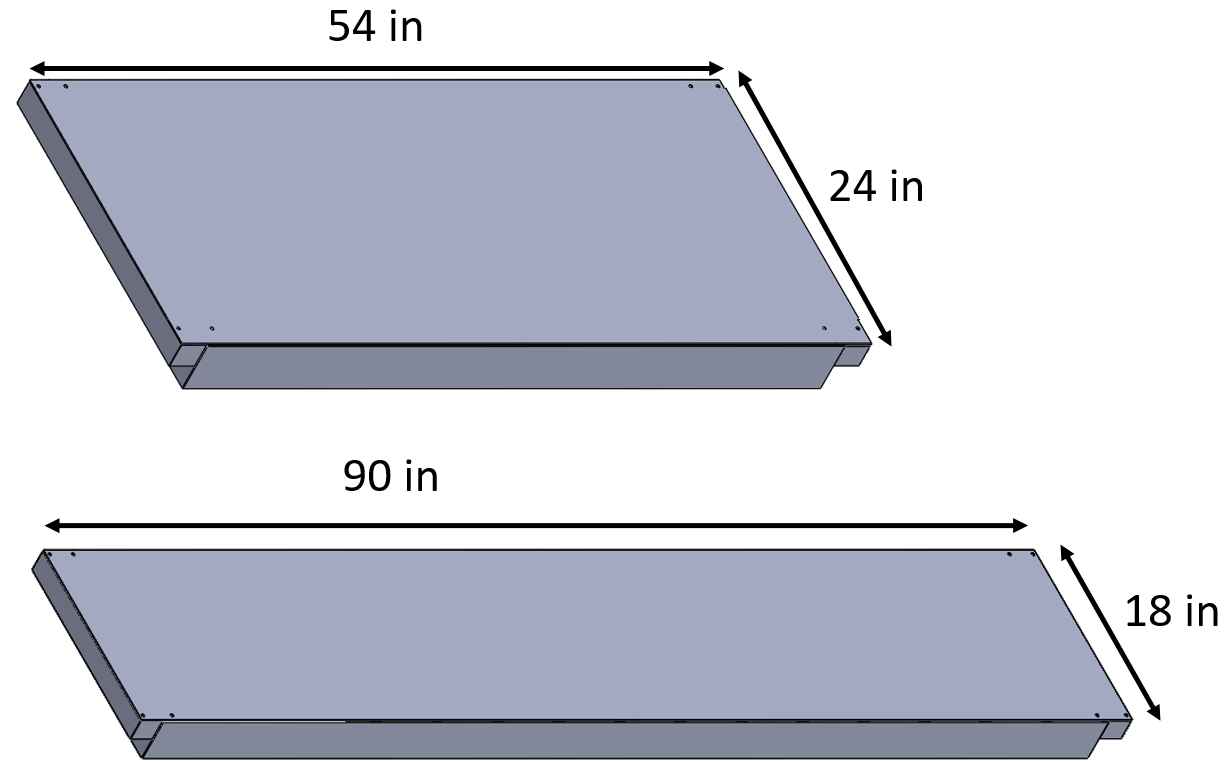
\includegraphics[width=0.75\textwidth]{ExampleRoofPanel}
\caption{Top: Conditioning section roof panel. Bottom: Test section roof panel.}
\label{fig:ExampleRoofPanel}
\end{figure}

\begin{figure} [h!]
\centering
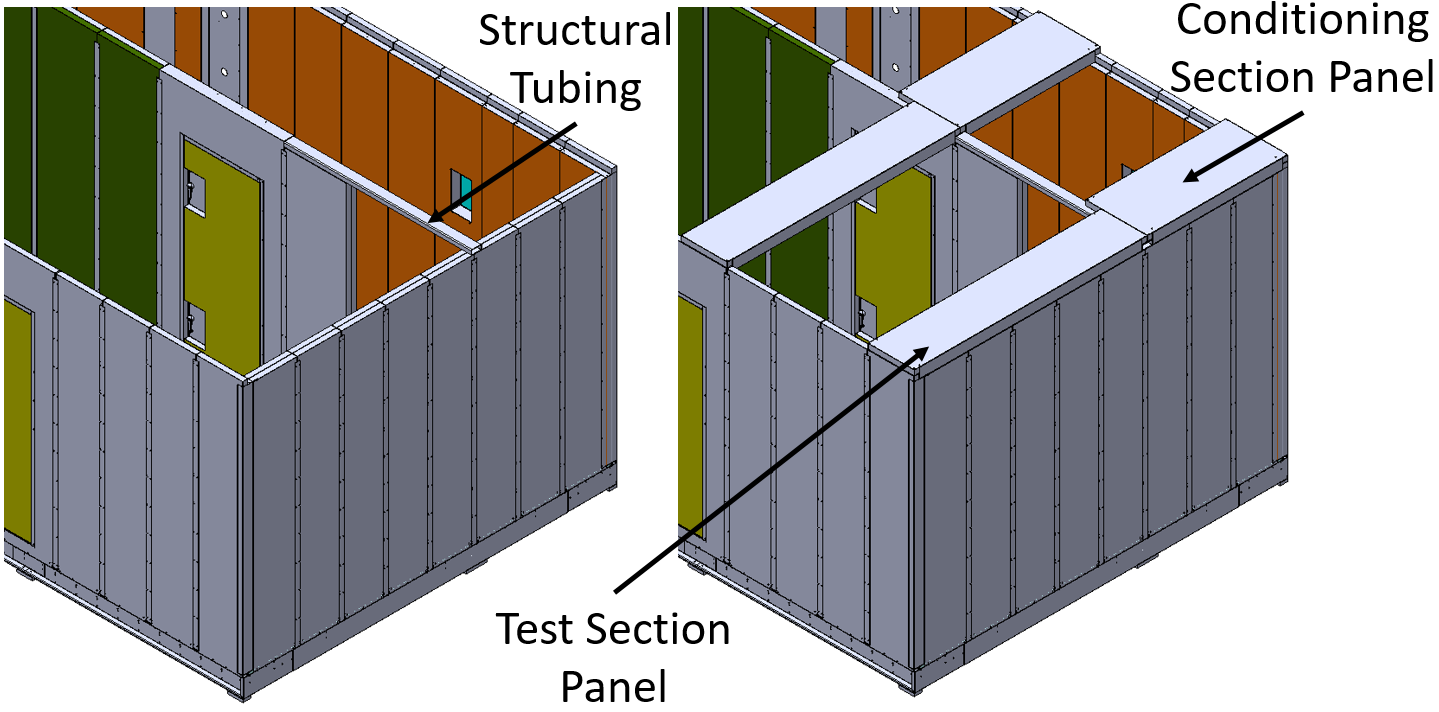
\includegraphics[width=1\textwidth]{RoofPanelPlacementCompIso}
\caption{Left: Placement of structural tubing for roof panel support. Right: Example of roof panel placement in isometric view.}
\label{fig:RoofPanelPlacementCompIso}
\end{figure}

\begin{figure} [h!]
\centering
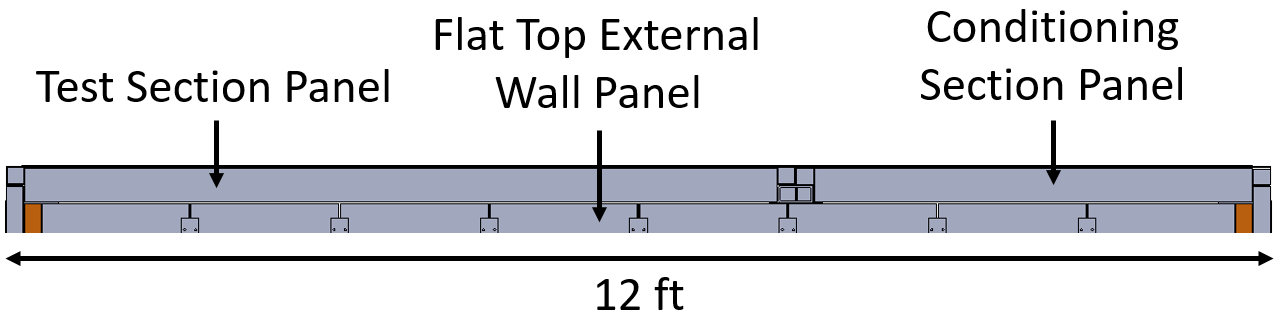
\includegraphics[width=1\textwidth]{RoofPanelPlacementCross}
\caption{Example of roof panel placement in cross sectional view.}
\label{fig:RoofPanelPlacementCross}
\end{figure}

\FloatBarrier

Roof panels are placed along the length of the walls. Figure \ref{fig:ClosedCabin} shows the final placement of all panels together. Access panels located on the roof are to be used for PIV in the future. 

\begin{figure} [h!]
\centering
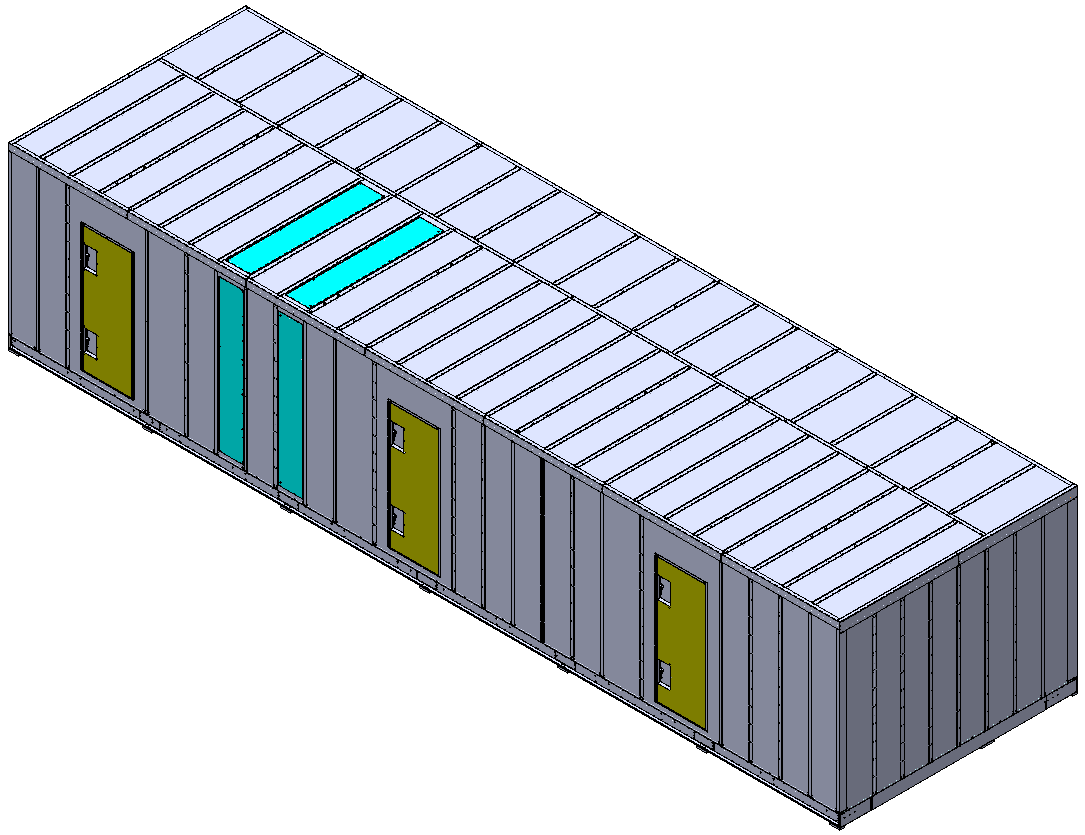
\includegraphics[width=1\textwidth]{ClosedCabin}
\caption{Final arrangement of all panels for the airside subsystem.}
\label{fig:ClosedCabin}
\end{figure}
